%%%%%%%%%%%%%%%%%%%%%%%%%%%%%%%%%%%%%%%%%%%%%%%%%%%%%%%%%%%%%%%%%%%%%%%%%%%%%%%%%%%%%%%%%%%%%%%%%%%%%%%%%%%%%%%%%%%%%%%%%%%%%%%%%%%%%%%%%%%%%%%%%%%%%%%%%%%%%%%%%%%
% Written By Michael Brodskiy
% Class: Fundamentals of Electronics
% Professor: M. Onabajo
%%%%%%%%%%%%%%%%%%%%%%%%%%%%%%%%%%%%%%%%%%%%%%%%%%%%%%%%%%%%%%%%%%%%%%%%%%%%%%%%%%%%%%%%%%%%%%%%%%%%%%%%%%%%%%%%%%%%%%%%%%%%%%%%%%%%%%%%%%%%%%%%%%%%%%%%%%%%%%%%%%%

\documentclass[12pt]{article} 
\usepackage{alphalph}
\usepackage[utf8]{inputenc}
\usepackage[russian,english]{babel}
\usepackage{titling}
\usepackage{amsmath}
\usepackage{graphicx}
\usepackage{enumitem}
\usepackage{amssymb}
\usepackage[super]{nth}
\usepackage{everysel}
\usepackage{ragged2e}
\usepackage{geometry}
\usepackage{multicol}
\usepackage{fancyhdr}
\usepackage{cancel}
\usepackage{siunitx}
\usepackage{physics}
\usepackage{tikz}
\usepackage{mathdots}
\usepackage{yhmath}
\usepackage{cancel}
\usepackage{color}
\usepackage{array}
\usepackage{multirow}
\usepackage{gensymb}
\usepackage{tabularx}
\usepackage{extarrows}
\usepackage{booktabs}
\usepackage{lastpage}
\usetikzlibrary{fadings}
\usetikzlibrary{patterns}
\usetikzlibrary{shadows.blur}
\usetikzlibrary{shapes}

\geometry{top=1.0in,bottom=1.0in,left=1.0in,right=1.0in}
\newcommand{\subtitle}[1]{%
  \posttitle{%
    \par\end{center}
    \begin{center}\large#1\end{center}
    \vskip0.5em}%

}
\usepackage{hyperref}
\hypersetup{
colorlinks=true,
linkcolor=blue,
filecolor=magenta,      
urlcolor=blue,
citecolor=blue,
}


\title{Homework 3}
\date{\today}
\author{Michael Brodskiy\\ \small Professor: M. Onabajo}

\begin{document}

\maketitle

\begin{enumerate}

  \item The following plots can be made for $i$ versus $V$ of the given circuits:

    \begin{enumerate}

      \item Circuit 1:

        \begin{figure}[H]
          \centering
          \tikzset{every picture/.style={line width=0.75pt}} %set default line width to 0.75pt        

\begin{tikzpicture}[x=0.75pt,y=0.75pt,yscale=-.75,xscale=.75]
%uncomment if require: \path (0,692); %set diagram left start at 0, and has height of 692

%Shape: Axis 2D [id:dp7787745858917079] 
\draw  (270,336.6) -- (574,336.6)(300.4,63) -- (300.4,367) (567,331.6) -- (574,336.6) -- (567,341.6) (295.4,70) -- (300.4,63) -- (305.4,70)  ;
%Shape: Axis 2D [id:dp2833357045793793] 
\draw  (330.8,336.6) -- (26.8,336.6)(300.4,63) -- (300.4,367) (33.8,331.6) -- (26.8,336.6) -- (33.8,341.6) (305.4,70) -- (300.4,63) -- (295.4,70)  ;
%Shape: Grid [id:dp29542181740302487] 
\draw  [draw opacity=0][dash pattern={on 4.5pt off 4.5pt}] (60,97) -- (300.4,97) -- (300.4,335.7) -- (60,335.7) -- cycle ; \draw  [color={rgb, 255:red, 155; green, 155; blue, 155 }  ,draw opacity=1 ][dash pattern={on 4.5pt off 4.5pt}] (60,97) -- (60,335.7)(120,97) -- (120,335.7)(180,97) -- (180,335.7)(240,97) -- (240,335.7)(300,97) -- (300,335.7) ; \draw  [color={rgb, 255:red, 155; green, 155; blue, 155 }  ,draw opacity=1 ][dash pattern={on 4.5pt off 4.5pt}] (60,97) -- (300.4,97)(60,157) -- (300.4,157)(60,217) -- (300.4,217)(60,277) -- (300.4,277) ; \draw  [color={rgb, 255:red, 155; green, 155; blue, 155 }  ,draw opacity=1 ][dash pattern={on 4.5pt off 4.5pt}]  ;
%Shape: Grid [id:dp6629033718892944] 
\draw  [draw opacity=0][dash pattern={on 4.5pt off 4.5pt}] (540,97) -- (299.6,97) -- (299.6,335) -- (540,335) -- cycle ; \draw  [color={rgb, 255:red, 155; green, 155; blue, 155 }  ,draw opacity=1 ][dash pattern={on 4.5pt off 4.5pt}] (540,97) -- (540,335)(480,97) -- (480,335)(420,97) -- (420,335)(360,97) -- (360,335)(300,97) -- (300,335) ; \draw  [color={rgb, 255:red, 155; green, 155; blue, 155 }  ,draw opacity=1 ][dash pattern={on 4.5pt off 4.5pt}] (540,97) -- (299.6,97)(540,157) -- (299.6,157)(540,217) -- (299.6,217)(540,277) -- (299.6,277) ; \draw  [color={rgb, 255:red, 155; green, 155; blue, 155 }  ,draw opacity=1 ][dash pattern={on 4.5pt off 4.5pt}]  ;
%Shape: Axis 2D [id:dp05057739971766584] 
\draw  (270,336.4) -- (574,336.4)(300.4,610) -- (300.4,306) (567,341.4) -- (574,336.4) -- (567,331.4) (295.4,603) -- (300.4,610) -- (305.4,603)  ;
%Shape: Axis 2D [id:dp7802415405732975] 
\draw  (330.8,336.4) -- (26.8,336.4)(300.4,610) -- (300.4,306) (33.8,341.4) -- (26.8,336.4) -- (33.8,331.4) (305.4,603) -- (300.4,610) -- (295.4,603)  ;
%Shape: Grid [id:dp6823563734954645] 
\draw  [draw opacity=0][dash pattern={on 4.5pt off 4.5pt}] (60,576) -- (300.4,576) -- (300.4,337.3) -- (60,337.3) -- cycle ; \draw  [color={rgb, 255:red, 155; green, 155; blue, 155 }  ,draw opacity=1 ][dash pattern={on 4.5pt off 4.5pt}] (60,576) -- (60,337.3)(120,576) -- (120,337.3)(180,576) -- (180,337.3)(240,576) -- (240,337.3)(300,576) -- (300,337.3) ; \draw  [color={rgb, 255:red, 155; green, 155; blue, 155 }  ,draw opacity=1 ][dash pattern={on 4.5pt off 4.5pt}] (60,576) -- (300.4,576)(60,516) -- (300.4,516)(60,456) -- (300.4,456)(60,396) -- (300.4,396) ; \draw  [color={rgb, 255:red, 155; green, 155; blue, 155 }  ,draw opacity=1 ][dash pattern={on 4.5pt off 4.5pt}]  ;
%Shape: Grid [id:dp350033892870824] 
\draw  [draw opacity=0][dash pattern={on 4.5pt off 4.5pt}] (540,576) -- (299.6,576) -- (299.6,338) -- (540,338) -- cycle ; \draw  [color={rgb, 255:red, 155; green, 155; blue, 155 }  ,draw opacity=1 ][dash pattern={on 4.5pt off 4.5pt}] (540,576) -- (540,338)(480,576) -- (480,338)(420,576) -- (420,338)(360,576) -- (360,338)(300,576) -- (300,338) ; \draw  [color={rgb, 255:red, 155; green, 155; blue, 155 }  ,draw opacity=1 ][dash pattern={on 4.5pt off 4.5pt}] (540,576) -- (299.6,576)(540,516) -- (299.6,516)(540,456) -- (299.6,456)(540,396) -- (299.6,396) ; \draw  [color={rgb, 255:red, 155; green, 155; blue, 155 }  ,draw opacity=1 ][dash pattern={on 4.5pt off 4.5pt}]  ;
%Shape: Arc [id:dp8040069079724227] 
\draw  [draw opacity=0][line width=1.5]  (120.11,363.39) .. controls (121.44,348.04) and (134.31,336) .. (150,336) -- (150,366) -- cycle ; \draw  [color={rgb, 255:red, 208; green, 2; blue, 27 }  ,draw opacity=1 ][line width=1.5]  (120.11,363.39) .. controls (121.44,348.04) and (134.31,336) .. (150,336) ;  
%Straight Lines [id:da010539851374448572] 
\draw [color={rgb, 255:red, 208; green, 2; blue, 27 }  ,draw opacity=1 ][line width=1.5]    (100.38,588.94) -- (120.11,363.39) ;
%Straight Lines [id:da5534986179467353] 
\draw [color={rgb, 255:red, 208; green, 2; blue, 27 }  ,draw opacity=1 ][line width=1.5]    (150,336) -- (450,337) ;
%Shape: Arc [id:dp24170882699850038] 
\draw  [draw opacity=0][line width=1.5]  (479.89,309.61) .. controls (478.56,324.96) and (465.69,337) .. (450,337) -- (450,307) -- cycle ; \draw  [color={rgb, 255:red, 208; green, 2; blue, 27 }  ,draw opacity=1 ][line width=1.5]  (479.89,309.61) .. controls (478.56,324.96) and (465.69,337) .. (450,337) ;  
%Straight Lines [id:da6891777969315377] 
\draw [color={rgb, 255:red, 208; green, 2; blue, 27 }  ,draw opacity=1 ][line width=1.5]    (479.89,309.61) -- (499.62,84.06) ;
%Straight Lines [id:da966199825040796] 
\draw [line width=1.5]    (480,329.29) -- (480,343.71) ;
%Straight Lines [id:da8958941331400883] 
\draw [line width=1.5]    (120,330.29) -- (120,344.71) ;

% Text Node
\draw (264,59) node [anchor=south west] [inner sep=0.75pt]    {$i\left(\text{mA}\right)$};
% Text Node
\draw (577,348) node [anchor=south west] [inner sep=0.75pt]    {$V\left(\text{V}\right)$};
% Text Node
\draw (120,326.89) node [anchor=south] [inner sep=0.75pt]    {$-.6\left[\text{V}\right]$};
% Text Node
\draw (480,347.11) node [anchor=north] [inner sep=0.75pt]    {$.6\left[\text{V}\right]$};


\end{tikzpicture}

          \caption{Plot Showing Current-Voltage Relationship for Circuit 1}
          \label{fig:1}
        \end{figure}
        
      \item Circuit 2 (we obtain the voltage values by summing $.6+6.8=7.4[\si{\volt}]$). Note, there is only a positive voltage response since a forward-biased diode is placed:

        \begin{figure}[H]
          \centering
          \tikzset{every picture/.style={line width=0.75pt}} %set default line width to 0.75pt        

\begin{tikzpicture}[x=0.75pt,y=0.75pt,yscale=-.75,xscale=.75]
%uncomment if require: \path (0,692); %set diagram left start at 0, and has height of 692

%Shape: Axis 2D [id:dp7787745858917079] 
\draw  (270,336.6) -- (574,336.6)(300.4,63) -- (300.4,367) (567,331.6) -- (574,336.6) -- (567,341.6) (295.4,70) -- (300.4,63) -- (305.4,70)  ;
%Shape: Axis 2D [id:dp2833357045793793] 
\draw  (330.8,336.6) -- (26.8,336.6)(300.4,63) -- (300.4,367) (33.8,331.6) -- (26.8,336.6) -- (33.8,341.6) (305.4,70) -- (300.4,63) -- (295.4,70)  ;
%Shape: Grid [id:dp29542181740302487] 
\draw  [draw opacity=0][dash pattern={on 4.5pt off 4.5pt}] (60,97) -- (300.4,97) -- (300.4,335.7) -- (60,335.7) -- cycle ; \draw  [color={rgb, 255:red, 155; green, 155; blue, 155 }  ,draw opacity=1 ][dash pattern={on 4.5pt off 4.5pt}] (60,97) -- (60,335.7)(120,97) -- (120,335.7)(180,97) -- (180,335.7)(240,97) -- (240,335.7)(300,97) -- (300,335.7) ; \draw  [color={rgb, 255:red, 155; green, 155; blue, 155 }  ,draw opacity=1 ][dash pattern={on 4.5pt off 4.5pt}] (60,97) -- (300.4,97)(60,157) -- (300.4,157)(60,217) -- (300.4,217)(60,277) -- (300.4,277) ; \draw  [color={rgb, 255:red, 155; green, 155; blue, 155 }  ,draw opacity=1 ][dash pattern={on 4.5pt off 4.5pt}]  ;
%Shape: Grid [id:dp6629033718892944] 
\draw  [draw opacity=0][dash pattern={on 4.5pt off 4.5pt}] (540,97) -- (299.6,97) -- (299.6,335) -- (540,335) -- cycle ; \draw  [color={rgb, 255:red, 155; green, 155; blue, 155 }  ,draw opacity=1 ][dash pattern={on 4.5pt off 4.5pt}] (540,97) -- (540,335)(480,97) -- (480,335)(420,97) -- (420,335)(360,97) -- (360,335)(300,97) -- (300,335) ; \draw  [color={rgb, 255:red, 155; green, 155; blue, 155 }  ,draw opacity=1 ][dash pattern={on 4.5pt off 4.5pt}] (540,97) -- (299.6,97)(540,157) -- (299.6,157)(540,217) -- (299.6,217)(540,277) -- (299.6,277) ; \draw  [color={rgb, 255:red, 155; green, 155; blue, 155 }  ,draw opacity=1 ][dash pattern={on 4.5pt off 4.5pt}]  ;
%Shape: Axis 2D [id:dp05057739971766584] 
\draw  (270,336.4) -- (574,336.4)(300.4,610) -- (300.4,306) (567,341.4) -- (574,336.4) -- (567,331.4) (295.4,603) -- (300.4,610) -- (305.4,603)  ;
%Shape: Axis 2D [id:dp7802415405732975] 
\draw  (330.8,336.4) -- (26.8,336.4)(300.4,610) -- (300.4,306) (33.8,341.4) -- (26.8,336.4) -- (33.8,331.4) (305.4,603) -- (300.4,610) -- (295.4,603)  ;
%Shape: Grid [id:dp6823563734954645] 
\draw  [draw opacity=0][dash pattern={on 4.5pt off 4.5pt}] (60,576) -- (300.4,576) -- (300.4,337.3) -- (60,337.3) -- cycle ; \draw  [color={rgb, 255:red, 155; green, 155; blue, 155 }  ,draw opacity=1 ][dash pattern={on 4.5pt off 4.5pt}] (60,576) -- (60,337.3)(120,576) -- (120,337.3)(180,576) -- (180,337.3)(240,576) -- (240,337.3)(300,576) -- (300,337.3) ; \draw  [color={rgb, 255:red, 155; green, 155; blue, 155 }  ,draw opacity=1 ][dash pattern={on 4.5pt off 4.5pt}] (60,576) -- (300.4,576)(60,516) -- (300.4,516)(60,456) -- (300.4,456)(60,396) -- (300.4,396) ; \draw  [color={rgb, 255:red, 155; green, 155; blue, 155 }  ,draw opacity=1 ][dash pattern={on 4.5pt off 4.5pt}]  ;
%Shape: Grid [id:dp350033892870824] 
\draw  [draw opacity=0][dash pattern={on 4.5pt off 4.5pt}] (540,576) -- (299.6,576) -- (299.6,338) -- (540,338) -- cycle ; \draw  [color={rgb, 255:red, 155; green, 155; blue, 155 }  ,draw opacity=1 ][dash pattern={on 4.5pt off 4.5pt}] (540,576) -- (540,338)(480,576) -- (480,338)(420,576) -- (420,338)(360,576) -- (360,338)(300,576) -- (300,338) ; \draw  [color={rgb, 255:red, 155; green, 155; blue, 155 }  ,draw opacity=1 ][dash pattern={on 4.5pt off 4.5pt}] (540,576) -- (299.6,576)(540,516) -- (299.6,516)(540,456) -- (299.6,456)(540,396) -- (299.6,396) ; \draw  [color={rgb, 255:red, 155; green, 155; blue, 155 }  ,draw opacity=1 ][dash pattern={on 4.5pt off 4.5pt}]  ;
%Straight Lines [id:da5534986179467353] 
\draw [color={rgb, 255:red, 208; green, 2; blue, 27 }  ,draw opacity=1 ][line width=1.5]    (36,336) -- (450,337) ;
%Shape: Arc [id:dp24170882699850038] 
\draw  [draw opacity=0][line width=1.5]  (479.89,309.61) .. controls (478.56,324.96) and (465.69,337) .. (450,337) -- (450,307) -- cycle ; \draw  [color={rgb, 255:red, 208; green, 2; blue, 27 }  ,draw opacity=1 ][line width=1.5]  (479.89,309.61) .. controls (478.56,324.96) and (465.69,337) .. (450,337) ;  
%Straight Lines [id:da6891777969315377] 
\draw [color={rgb, 255:red, 208; green, 2; blue, 27 }  ,draw opacity=1 ][line width=1.5]    (479.89,309.61) -- (499.62,84.06) ;
%Straight Lines [id:da966199825040796] 
\draw [line width=1.5]    (480,329.29) -- (480,343.71) ;

% Text Node
\draw (264,59) node [anchor=south west] [inner sep=0.75pt]    {$i\left(\text{mA}\right)$};
% Text Node
\draw (577,348) node [anchor=south west] [inner sep=0.75pt]    {$V\left(\text{V}\right)$};
% Text Node
\draw (480,347.11) node [anchor=north] [inner sep=0.75pt]    {$7.4\left[\text{V}\right]$};


\end{tikzpicture}

          \caption{Plot Showing Current-Voltage Relationship for Circuit 2}
          \label{fig:2}
        \end{figure}
        
      \item Circuit 3 (we obtain the voltage values by summing $5.6+.6=6.2[\si{\volt}]$):
        
        \begin{figure}[H]
          \centering
          \tikzset{every picture/.style={line width=0.75pt}} %set default line width to 0.75pt        

\begin{tikzpicture}[x=0.75pt,y=0.75pt,yscale=-.75,xscale=.75]
%uncomment if require: \path (0,692); %set diagram left start at 0, and has height of 692

%Shape: Axis 2D [id:dp7787745858917079] 
\draw  (270,336.6) -- (574,336.6)(300.4,63) -- (300.4,367) (567,331.6) -- (574,336.6) -- (567,341.6) (295.4,70) -- (300.4,63) -- (305.4,70)  ;
%Shape: Axis 2D [id:dp2833357045793793] 
\draw  (330.8,336.6) -- (26.8,336.6)(300.4,63) -- (300.4,367) (33.8,331.6) -- (26.8,336.6) -- (33.8,341.6) (305.4,70) -- (300.4,63) -- (295.4,70)  ;
%Shape: Grid [id:dp29542181740302487] 
\draw  [draw opacity=0][dash pattern={on 4.5pt off 4.5pt}] (60,97) -- (300.4,97) -- (300.4,335.7) -- (60,335.7) -- cycle ; \draw  [color={rgb, 255:red, 155; green, 155; blue, 155 }  ,draw opacity=1 ][dash pattern={on 4.5pt off 4.5pt}] (60,97) -- (60,335.7)(120,97) -- (120,335.7)(180,97) -- (180,335.7)(240,97) -- (240,335.7)(300,97) -- (300,335.7) ; \draw  [color={rgb, 255:red, 155; green, 155; blue, 155 }  ,draw opacity=1 ][dash pattern={on 4.5pt off 4.5pt}] (60,97) -- (300.4,97)(60,157) -- (300.4,157)(60,217) -- (300.4,217)(60,277) -- (300.4,277) ; \draw  [color={rgb, 255:red, 155; green, 155; blue, 155 }  ,draw opacity=1 ][dash pattern={on 4.5pt off 4.5pt}]  ;
%Shape: Grid [id:dp6629033718892944] 
\draw  [draw opacity=0][dash pattern={on 4.5pt off 4.5pt}] (540,97) -- (299.6,97) -- (299.6,335) -- (540,335) -- cycle ; \draw  [color={rgb, 255:red, 155; green, 155; blue, 155 }  ,draw opacity=1 ][dash pattern={on 4.5pt off 4.5pt}] (540,97) -- (540,335)(480,97) -- (480,335)(420,97) -- (420,335)(360,97) -- (360,335)(300,97) -- (300,335) ; \draw  [color={rgb, 255:red, 155; green, 155; blue, 155 }  ,draw opacity=1 ][dash pattern={on 4.5pt off 4.5pt}] (540,97) -- (299.6,97)(540,157) -- (299.6,157)(540,217) -- (299.6,217)(540,277) -- (299.6,277) ; \draw  [color={rgb, 255:red, 155; green, 155; blue, 155 }  ,draw opacity=1 ][dash pattern={on 4.5pt off 4.5pt}]  ;
%Shape: Axis 2D [id:dp05057739971766584] 
\draw  (270,336.4) -- (574,336.4)(300.4,610) -- (300.4,306) (567,341.4) -- (574,336.4) -- (567,331.4) (295.4,603) -- (300.4,610) -- (305.4,603)  ;
%Shape: Axis 2D [id:dp7802415405732975] 
\draw  (330.8,336.4) -- (26.8,336.4)(300.4,610) -- (300.4,306) (33.8,341.4) -- (26.8,336.4) -- (33.8,331.4) (305.4,603) -- (300.4,610) -- (295.4,603)  ;
%Shape: Grid [id:dp6823563734954645] 
\draw  [draw opacity=0][dash pattern={on 4.5pt off 4.5pt}] (60,576) -- (300.4,576) -- (300.4,337.3) -- (60,337.3) -- cycle ; \draw  [color={rgb, 255:red, 155; green, 155; blue, 155 }  ,draw opacity=1 ][dash pattern={on 4.5pt off 4.5pt}] (60,576) -- (60,337.3)(120,576) -- (120,337.3)(180,576) -- (180,337.3)(240,576) -- (240,337.3)(300,576) -- (300,337.3) ; \draw  [color={rgb, 255:red, 155; green, 155; blue, 155 }  ,draw opacity=1 ][dash pattern={on 4.5pt off 4.5pt}] (60,576) -- (300.4,576)(60,516) -- (300.4,516)(60,456) -- (300.4,456)(60,396) -- (300.4,396) ; \draw  [color={rgb, 255:red, 155; green, 155; blue, 155 }  ,draw opacity=1 ][dash pattern={on 4.5pt off 4.5pt}]  ;
%Shape: Grid [id:dp350033892870824] 
\draw  [draw opacity=0][dash pattern={on 4.5pt off 4.5pt}] (540,576) -- (299.6,576) -- (299.6,338) -- (540,338) -- cycle ; \draw  [color={rgb, 255:red, 155; green, 155; blue, 155 }  ,draw opacity=1 ][dash pattern={on 4.5pt off 4.5pt}] (540,576) -- (540,338)(480,576) -- (480,338)(420,576) -- (420,338)(360,576) -- (360,338)(300,576) -- (300,338) ; \draw  [color={rgb, 255:red, 155; green, 155; blue, 155 }  ,draw opacity=1 ][dash pattern={on 4.5pt off 4.5pt}] (540,576) -- (299.6,576)(540,516) -- (299.6,516)(540,456) -- (299.6,456)(540,396) -- (299.6,396) ; \draw  [color={rgb, 255:red, 155; green, 155; blue, 155 }  ,draw opacity=1 ][dash pattern={on 4.5pt off 4.5pt}]  ;
%Shape: Arc [id:dp8040069079724227] 
\draw  [draw opacity=0][line width=1.5]  (120.11,363.39) .. controls (121.44,348.04) and (134.31,336) .. (150,336) -- (150,366) -- cycle ; \draw  [color={rgb, 255:red, 208; green, 2; blue, 27 }  ,draw opacity=1 ][line width=1.5]  (120.11,363.39) .. controls (121.44,348.04) and (134.31,336) .. (150,336) ;  
%Straight Lines [id:da010539851374448572] 
\draw [color={rgb, 255:red, 208; green, 2; blue, 27 }  ,draw opacity=1 ][line width=1.5]    (100.38,588.94) -- (120.11,363.39) ;
%Straight Lines [id:da5534986179467353] 
\draw [color={rgb, 255:red, 208; green, 2; blue, 27 }  ,draw opacity=1 ][line width=1.5]    (150,336) -- (450,337) ;
%Shape: Arc [id:dp24170882699850038] 
\draw  [draw opacity=0][line width=1.5]  (479.89,309.61) .. controls (478.56,324.96) and (465.69,337) .. (450,337) -- (450,307) -- cycle ; \draw  [color={rgb, 255:red, 208; green, 2; blue, 27 }  ,draw opacity=1 ][line width=1.5]  (479.89,309.61) .. controls (478.56,324.96) and (465.69,337) .. (450,337) ;  
%Straight Lines [id:da6891777969315377] 
\draw [color={rgb, 255:red, 208; green, 2; blue, 27 }  ,draw opacity=1 ][line width=1.5]    (479.89,309.61) -- (499.62,84.06) ;
%Straight Lines [id:da966199825040796] 
\draw [line width=1.5]    (480,329.29) -- (480,343.71) ;
%Straight Lines [id:da8958941331400883] 
\draw [line width=1.5]    (120,330.29) -- (120,344.71) ;

% Text Node
\draw (264,59) node [anchor=south west] [inner sep=0.75pt]    {$i\left(\text{mA}\right)$};
% Text Node
\draw (577,348) node [anchor=south west] [inner sep=0.75pt]    {$V\left(\text{V}\right)$};
% Text Node
\draw (120,326.89) node [anchor=south] [inner sep=0.75pt]    {$-6.2\left[\text{V}\right]$};
% Text Node
\draw (480,347.11) node [anchor=north] [inner sep=0.75pt]    {$6.2\left[\text{V}\right]$};


\end{tikzpicture}

          \caption{Plot Showing Current-Voltage Relationship for Circuit 3}
          \label{fig:3}
        \end{figure}
        
    \end{enumerate}

  \item

    \begin{enumerate}

      \item We begin assuming forward bias for both diodes, which gives a simple circuit with only resistors. This gives us a current from the source of:

        $$I_s=\frac{15}{2\left( \frac{(5k)(10k)}{15k} \right)}$$
        $$I_s=2.25[\si{\milli\ampere}]$$

        The current then splits into the branches. We can calculate the current across the first 10k and 5k resistors as:

        $$i_{5k}=\left( \frac{10}{15} \right)(2.25)$$
        $$i_{10k}=\left( \frac{5}{15} \right)(2.25)$$

        $$i_{5k}=1.5[\si{\milli\ampere}]$$
        $$i_{10k}=.75[\si{\milli\ampere}]$$

        Since there is a positive current through the branch containing $D_1$,\\ \underline{we know the first diode is forward-biased} (so voltage must be zero). Since the next set of parallel resistors has the same values as the first set, we know that the current flow will be the same. Thus, we can say that the current through $D_2$ is:

        $$I+i_{5k}=i_{10k}$$
        $$I=-.75[\si{\milli\ampere}]$$

        Since this value is less than zero, \underline{the second diode is reverse-biased}. We now change our assumptions and solve for the voltages. Since there are two branches with equivalent resistances of 15k, we know that the voltage will split such that the 10k resistor receives $10[\si{\volt}]$ and the 5k resistor receives $5[\si{\volt}]$. Thus, the voltage drop across $D_2$ is $5[\si{\volt}]$ and the current through each parallel connection is $1[\si{\milli\ampere}]$. The diodes may be tabulated as follows:

        \begin{center}
          \begin{tabular}[H]{|c|c|c|}
            \hline
            Diode & $V[\si{\volt}]$ & $I[\si{\milli\ampere}]$\\
            \hline
            $D_1$ & $0$ & $1$\\
            \hline
            $D_2$ & $5$ & 0\\
            \hline
          \end{tabular}
        \end{center}

        We observe the following values: $\boxed{V=10[\si{\volt}], I=0[\si{\milli\ampere}]}$

      \item 

        If both of the diodes are forward-biased, then two voltage sources would be in parallel; since this is not feasible, one must be on while the other is off. Since the problem asks for the current through the $D_1$ branch, let us assume it is forward-biased, while $D_2$ is reverse biased. This gives:

        $$I=\frac{6}{1k}$$
        $$\boxed{I=6[\si{\milli\ampere}]}$$

        Since the voltage is expended solely on the resistor, we estimate:

        $$\boxed{V=6[\si{\volt}]}$$

      \item 
    
        Let use begin by assuming both diodes are forward-biased. In this case, there are 15 volts at the positive node of the 2.2k resistor, and 15 volts across the 1.5k resistor. We may observe that at the negative node, there are -15 volts. This means the voltage drop across the 2.2k resistor is 30$[\si{\Volt}]$. We may solve for the current:

        $$V_{2.2k}=\frac{15-(-15)}{2.2}$$
        $$V_{2.2k}=13.636[\si{\milli\ampere}]$$

        The current through the 1.5k resistor may be found as well, as we know the voltage drop will be $30[\si{\volt}]$ as well:

        $$V_{2.2k}=\frac{15-(-15)}{1.5}$$
        $$V_{2.2k}=20[\si{\milli\ampere}]$$

        We can use this to solve for the current through $D_2$:

        $$I=20+13.636$$
        $$I=33.636[\si{\milli\ampere}]$$

        As such, our initial assumptions are correct, and our values of interest are:

        $$\boxed{V=30[\si{\volt}],\,I=33.636[\si{\milli\ampere}]}$$

    \end{enumerate}

  \item Repeat Problem 2, but using the Constant Voltage Drop (CVD) model with a voltage drop of $.7[\si{\volt}]$ for forward-biased diodes

    \begin{enumerate}

      \item 

        From 2(a), we know that $D_1$ is forward-biased, and $D_2$ is reverse-biased. This means that we can calculate the current through the branch as:

        $$i=\frac{15-.7}{15k}$$
        $$i=.9533[\si{\milli\ampere}]$$

        This gives:

        $$V=(.9533)(10)$$
        $$\boxed{V=9.533[\si{\volt}]}$$

        Since $D_2$ is still reverse-biased, the current remains $\boxed{I=0[\si{\ampere}]}$.

      \item 

        From 2(b), we know that $D_1$ is forward-biased, and $D_2$ is reverse-biased. This gives us the current as:

        $$I=\frac{6-.7}{1k}$$
        $$\boxed{I=5.3[\si{\milli\ampere}]}$$

        The voltage is then:

        $$V=6-.7$$
        $$\boxed{V=5.3[\si{\volt}]}$$

      \item 

        We know that both diodes are forward-biased. This means the voltage at the positive terminal of the 2.2k resistor is:

        $$V^+=15-.7$$
        $$V^+=14.3[\si{\volt}]$$

        And at the negative node it is:

        $$V^-=-15-.7$$
        $$V^-=-15.7[\si{\volt}]$$

        Thus, the voltage drop remains the same as previously observed $\boxed{V=30[\si{\volt}]}$. This means the current through both the 2.2k and the 1.5k resistor does not change, which implies the current stays the same as well:

        $$\boxed{I=33.636[\si{\milli\ampere}]}$$

    \end{enumerate}

  \item We can use the Shockley Equation to model this problem:

    $$I_D=I_S\left[ e^{\frac{V_D}{nV_T}} -1\right]$$

    Since $I_D/I_S>>1$, we can eliminate the $-1$, and write:

    $$\frac{I_D}{I_S}=e^{\frac{V_D}{nV_T}}$$

    Furthermore, we know that, at room temperature, the thermal voltage is:

    $$V_T\approx 25[\si{\milli\ampere}]$$

    we can now use the given equations to set up a system and solve.

    \begin{enumerate}

      \item 

        We begin by writing:

        $$\frac{5\cdot10^{-6}}{I_S}=e^{\frac{.5}{.025n}}$$
        $$\frac{10^{-4}}{I_S}=e^{\frac{.6}{.025n}}$$

        This allows us to write:

        $$10^{-4}e^{\frac{.6}{.025n}}=(5\cdot10^{-6})e^{\frac{.5}{.025n}}$$
        $$e^{-\frac{.6}{.025n}}=.05e^{-\frac{.5}{.025n}}$$
        $$e^{-\frac{4}{n}}=.05$$
        $$\frac{4}{n}=-\ln(.05)$$
        $$n=-\frac{4}{\ln(.05)}$$

        This gives us:

        $$\boxed{n=1.33}$$

      \item 

        We can go back and solve the equations using the obtained value of the emissions coefficient:

        $$I_S=10^{-4}e^{-\frac{.6}{(1.33)(.025)}}$$
        $$\boxed{I_S=1.5625\cdot10^{-12}[\si{\ampere}]}$$

        We can confirm our calculation by using the first equation:

        $$I_S=(5\cdot10^{-6})e^{-\frac{.5}{(1.33)(.025)}}$$

        $$\boxed{I_S=1.5625\cdot10^{-12}[\si{\ampere}]}$$

    \end{enumerate}

  \item

    We know that the sum of the voltages in the isolated loop containing the diode must sum to zero, which allows us to write:

    $$9.1-(28\cdot10^{-3})(5)-V_{zo}=0$$
    $$9.1-.14-V_{zo}=0$$
    $$\boxed{V_{zo}=8.96[\si{\volt}]}$$

    From here, we can apply the $10[\si{\milli\ampere}]$ test case:

    $$V_z=.01(5)+8.96$$
    $$\boxed{V_{z10[\si{\milli\ampere}]}=9.01[\si{\volt}]}$$

    And finally the $100[\si{\milli\ampere}]$ case:

    $$V_z=.1(5)+8.96$$
    $$\boxed{V_{z100[\si{\milli\ampere}]}=9.46[\si{\volt}]}$$

  \item

    \begin{enumerate}

      \item 

        Using $V_1=1.5[\si{\volt}]$, we may begin solving by removing the voltage drop resulting from $D_1$:

        $$V_2=(1.5-.7)[\si{\volt}]$$
        $$\boxed{V_2=.8[\si{\volt}]}$$

        For $D_3$ and $D_4$ to be forward biased, we need a minimum voltage of $2(.7)=1.4[\si{\volt}]$. Since $.8<1.4$, $D_3$ and $D_4$ are both reverse-biased, which results in a voltage of $\boxed{V_{out}=0[\si{\volt}]}$. Although not required, we can solve for $V_3$, since we know there will be a $.7[\si{\volt}]$ drop at $D_2$:

        $$V_{R1}=.8-.7$$
        $$V_{R1}=.1[\si{\volt}]$$
        $$V_3=V_2-V_{R1}$$
        $$\boxed{V_3=.7[\si{\volt}]}$$

      \item We build the schematic and obtain the voltage readings below:

        \begin{figure}[H]
          \centering
          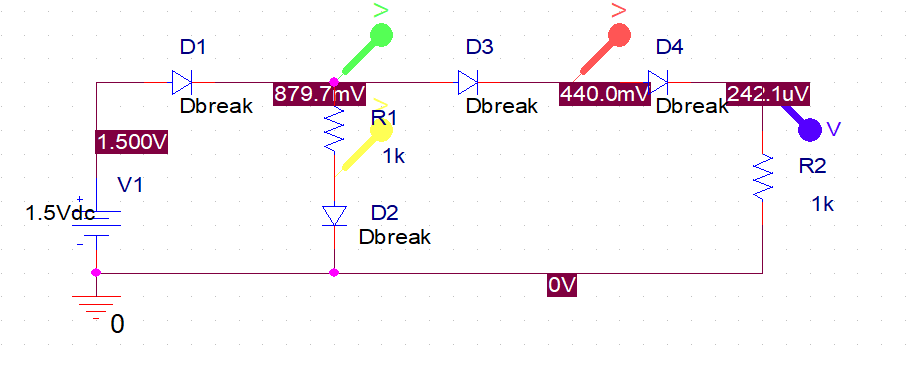
\includegraphics[width=.9\textwidth]{Figures/HW3Schem.png}
          \caption{Schematic with Corresponding Voltage Values (Note $V_{out}$ is Approximately $0[\si{\volt}]$)}
          \label{fig:4}
        \end{figure}

        \begin{figure}[H]
          \centering
          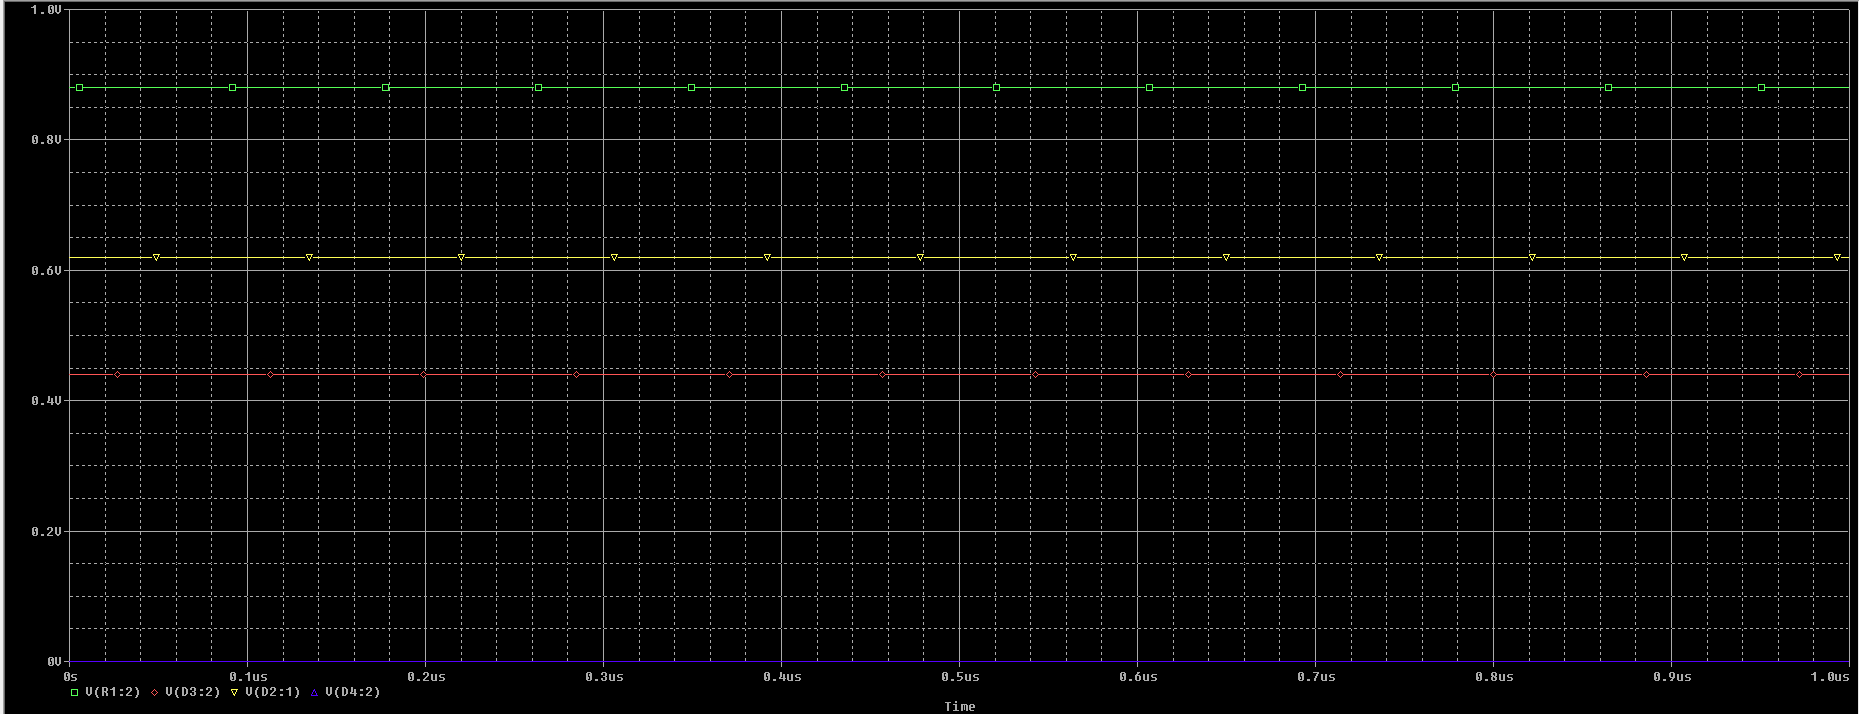
\includegraphics[width=.9\textwidth]{Figures/HW3-b.png}
          \caption{Plot Corresponding to Initial Simulation}
          \label{fig:5}
        \end{figure}

      \item Running the DC Sweep, we obtain:

        \begin{figure}[H]
          \centering
          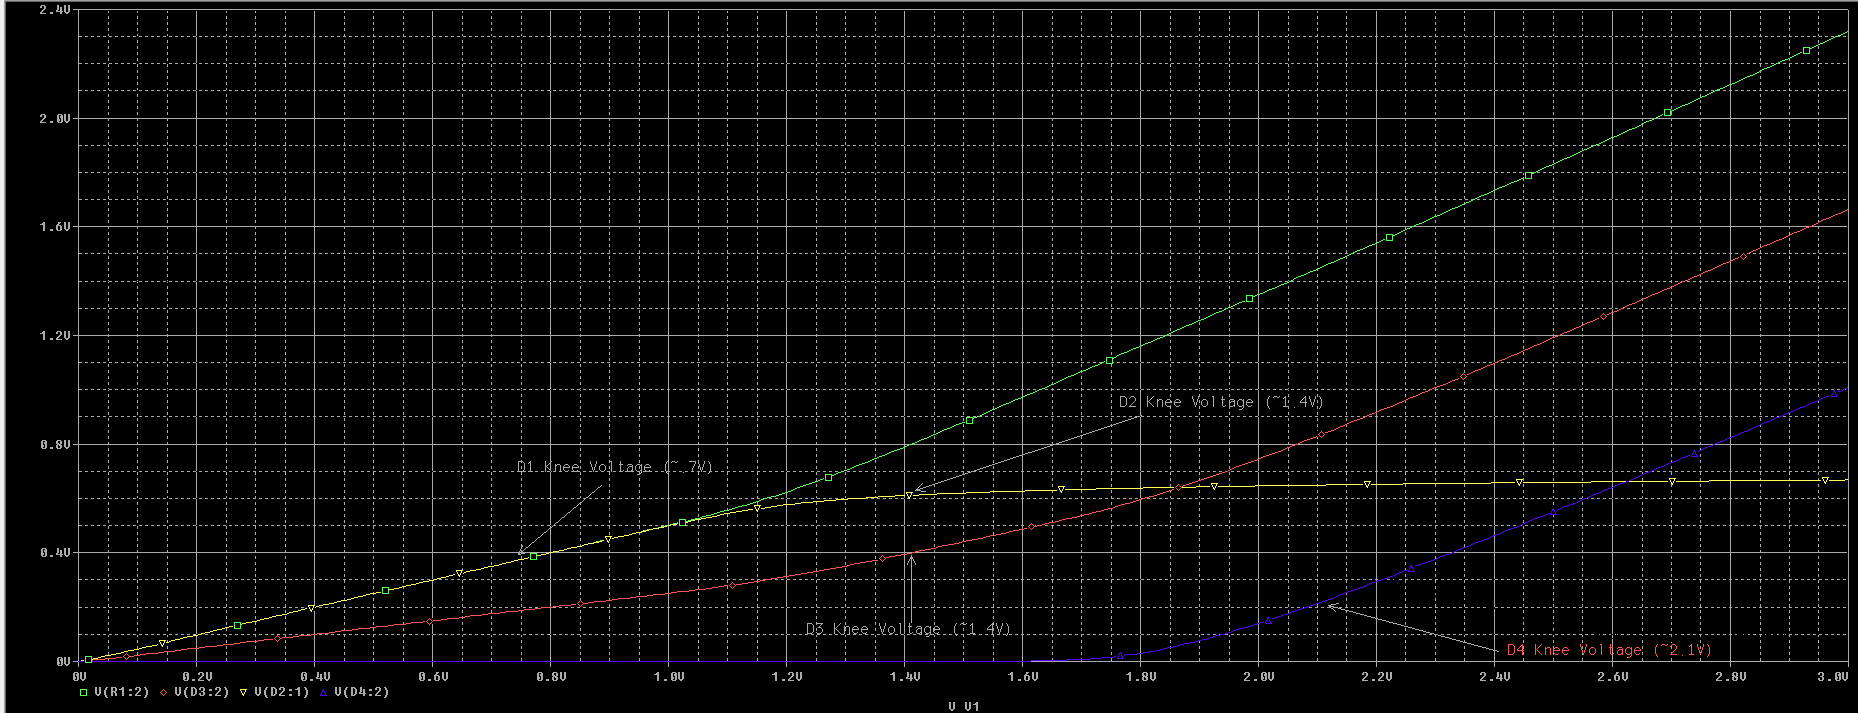
\includegraphics[width=.9\textwidth]{Figures/HW3-c.png}
          \caption{DC Sweep $0-3[\si{\volt}]$}
          \label{fig:6}
        \end{figure}

    \end{enumerate}

\end{enumerate}

\end{document}

